\section{TCP}
\subsection{Opgave 1}
\begin{figure}[H]
	\centering
	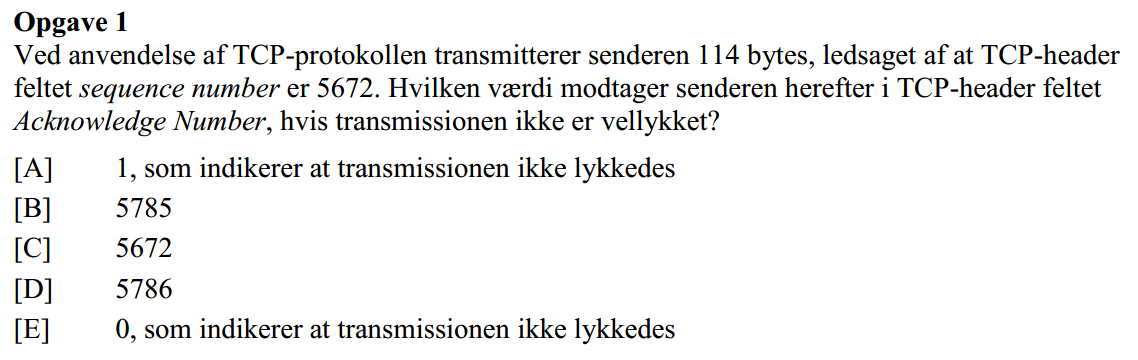
\includegraphics[width=\linewidth]{figs/tcp/SE15OP1}
\end{figure}

\begin{figure}[h]
	\centering
	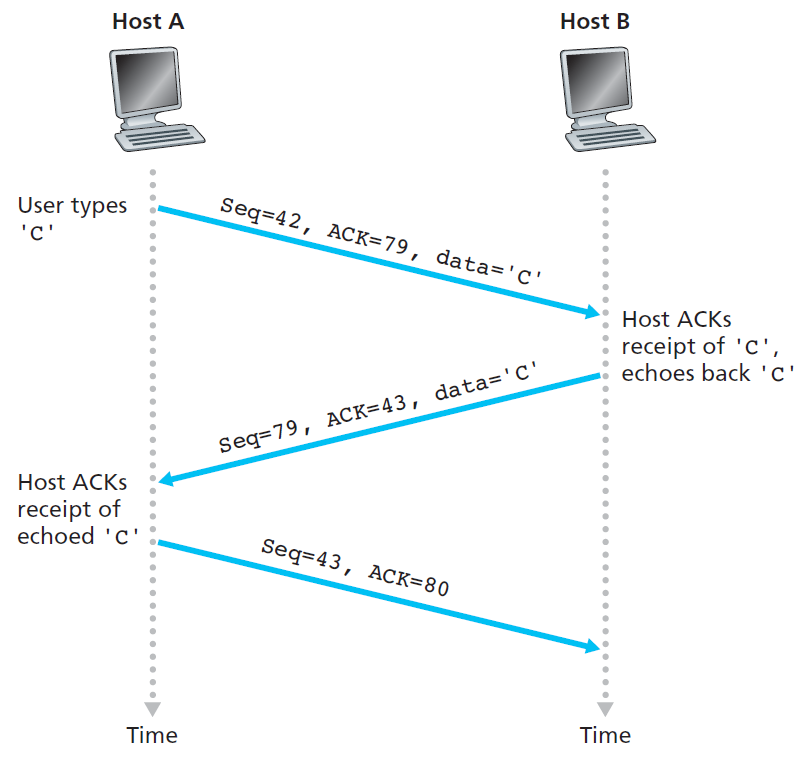
\includegraphics[width=0.8\textwidth]{figs/tcp/tcptransfer}
	\caption{Illustration af TCP transfer}
	\label{fig:TCPtransfer}
\end{figure}

\paragraph{[C]}Som det ses på figur \ref{fig:TCPtransfer} starter sequence number og acknowledge number på hhv. 42 og 79 (random genereret). SEQ og ACK inkrementeres med 1, skiftevis. Da transmissionen fejler, inkremeneteres der ikke.